\documentclass[a4paper,14pt]{extarticle}

% Русский язык
\usepackage{polyglossia}
\setdefaultlanguage{russian}

% Шрифты
\usepackage{fontspec}
\setmainfont{Times New Roman}
\setmonofont{Courier New} % моноширинный для кода

% Геометрия страницы 
\usepackage[left=30mm,right=15mm,top=20mm,bottom=20mm]{geometry}

% Математика, рисунки, подписи 
\usepackage{amsmath,amssymb}
\usepackage{graphicx}
\usepackage{float}
\usepackage{caption}

% Код 
\usepackage{listings}
\usepackage{xcolor}

\lstset{
  basicstyle=\ttfamily\small,
  breaklines=true,
  frame=single,
  columns=fullflexible,
  keepspaces=true,
  showstringspaces=false,
  tabsize=4
}

\captionsetup{labelsep=colon}

\begin{document}


% ТИТУЛЬНЫЙ ЛИСТ

\begin{center}

\textbf{МИНИСТЕРСТВО НАУКИ И ВЫСШЕГО ОБРАЗОВАНИЯ\\
РОССИЙСКОЙ ФЕДЕРАЦИИ}

\vspace{0.6cm}

\textbf{ФЕДЕРАЛЬНОЕ ГОСУДАРСТВЕННОЕ БЮДЖЕТНОЕ\\
ОБРАЗОВАТЕЛЬНОЕ УЧРЕЖДЕНИЕ ВЫСШЕГО ОБРАЗОВАНИЯ\\
«БЕЛГОРОДСКИЙ ГОСУДАРСТВЕННЫЙ ТЕХНОЛОГИЧЕСКИЙ\\
УНИВЕРСИТЕТ им. В. Г. Шухова»\\
(БГТУ им. В. Г. Шухова)}


\vspace{0.6cm}


\includegraphics[width=0.22\textwidth]{logo.jpg}

\vspace{0.6cm}

Кафедра программного обеспечения вычислительной\\
техники и автоматизированных систем

\vspace{1.5cm}

\textbf{Лабораторная работа № 1}\\
по дисциплине: «Объектно-ориентированное программирование»\\
на тему «Исследование множества опорных планов системы ограничений\\
задачи линейного программирования (задачи ЛП) в канонической форме»

\vspace{2cm}

\begin{flushright}
Выполнил: ст. группы ПВ-242\\
Кладченко Никита Сергеевич

\vspace{0.8cm}

Проверил:\\
Вирченко Юрий Петрович
\end{flushright}

\vfill

Белгород, 2026

\end{center}

\newpage


% ЦЕЛЬ И ЗАДАНИЕ

\textbf{Цель работы:} изучить метод Гаусса–Жордана и операцию замещения, а также освоить их применение к отысканию множества допустимых базисных видов системы линейных уравнений и решению задачи линейного программирования простым перебором опорных решений.

\vspace{0.4cm}

\textbf{Задание:}
\begin{enumerate}
\item Составить программу для отыскания всех базисных видов системы линейных уравнений.
\item Организовать отбор опорных планов среди всех базисных решений, а также нахождение оптимального опорного плана методом прямого перебора. Целевая функция выбирается произвольно.
\item Решить одну из задач вручную (подготовить тестовые данные).
\item Вариант 8.
\\[0.3cm]
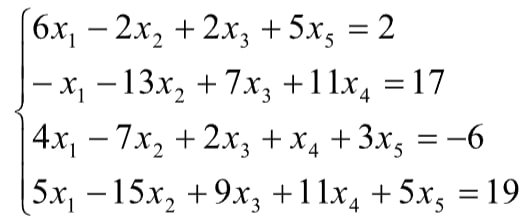
\includegraphics[
    width=0.6\textwidth,
    keepaspectratio
]{uslovie.jpg}
\end{enumerate}

\newpage


% ХОД РАБОТЫ

\section*{Ход работы}


% ЗАДАНИЕ 1

\section{Задание 1. Поиск всех базисных видов системы}

\subsection*{Код программы}
\begin{lstlisting}[language=Python]
from fractions import Fraction
from itertools import combinations

# Метод Гаусса-Жордана
def rref(matrix):
    A = [row[:] for row in matrix]

    rows = len(A)
    cols = len(A[0])

    r = 0
    c = 0
    pivots = []

    while r < rows and c < cols - 1:

        pivot = -1
        i = r
        while i < rows:
            if A[i][c] != 0:
                pivot = i
            i += 1

        if pivot == -1:
            c += 1
        else:
            A[r], A[pivot] = A[pivot], A[r]

            div = A[r][c]
            j = c
            while j < cols:
                A[r][j] /= div
                j += 1

            i = 0
            while i < rows:
                if i != r:
                    factor = A[i][c]
                    j = c
                    while j < cols:
                        A[i][j] -= factor * A[r][j]
                        j += 1
                i += 1

            pivots.append(c)
            r += 1
            c += 1

    return A, pivots


# Дано (вариант 8)
A = [
    [6, -2, 2, 0, 5],
    [-1, -13, 7, 11, 0],
    [4, -7, 2, 1, 3],
    [5, -15, 9, 11, 5]
]

b = [2, 17, -6, 19]

# перевод в дроби
for i in range(len(A)):
    for j in range(len(A[0])):
        A[i][j] = Fraction(A[i][j])
    b[i] = Fraction(b[i])

aug = [A[i] + [b[i]] for i in range(len(A))]

R, piv = rref(aug)

rank = len(piv)

print("([A|b]):\n")
for row in R:
    print(row)

print("\nРанг =", rank)

print("\nВсе базисные виды:\n")

for basis in combinations(range(5), rank):
    print("Базисные столбцы:", basis)
\end{lstlisting}

\subsection*{Блок-схемы программы}
\begin{figure}[H]
\centering

\includegraphics[width=0.55\textwidth]{MainEx1.png}
\caption{ Блок-схема main}
\end{figure}

\begin{figure}[H]
\centering

\includegraphics[width=0.85\textwidth]{RREFEx1.png}
\caption{ Начало блок-схемы функции rref}
\end{figure}

\begin{figure}[H]
\centering

\includegraphics[width=0.65\textwidth]{RREFEx1Continuation.png}
\caption{ Конец блок-схемы функции rref}
\end{figure}

\subsection*{Результат работы программы}
\begin{figure}[H]
\centering

\includegraphics[width=0.90\textwidth]{RezRabotyProg1.jpg}
\caption{ Результат работы программы 1}
\end{figure}

\newpage


% ЗАДАНИЕ 2

\section{Задание 2. Отбор опорных планов и поиск оптимального}

\subsection*{Код программы}
\begin{lstlisting}[language=Python]
from fractions import Fraction
from itertools import combinations


# решение системы
def solve(A, b):
    n = len(A)

    aug = []
    i = 0
    while i < n:
        aug.append(A[i][:] + [b[i]])
        i += 1

    r = 0
    c = 0

    while r < n and c < n:

        pivot = r
        while pivot < n and aug[pivot][c] == 0:
            pivot += 1

        if pivot < n:
            aug[r], aug[pivot] = aug[pivot], aug[r]

            div = aug[r][c]
            j = c
            while j <= n:
                aug[r][j] /= div
                j += 1

            i = 0
            while i < n:
                if i != r:
                    factor = aug[i][c]
                    j = c
                    while j <= n:
                        aug[i][j] -= factor * aug[r][j]
                        j += 1
                i += 1

            r += 1

        c += 1

    x = [Fraction(0)] * n
    i = 0
    while i < n:
        x[i] = aug[i][n]
        i += 1

    return x


# Дано (вариант 8)
A = [
    [6, -2, 2, 0, 5],
    [-1, -13, 7, 11, 0],
    [4, -7, 2, 1, 3],
    [5, -15, 9, 11, 5]
]

b = [2, 17, -6, 19]

m = 3  # ранг системы
n = 5

# целевая функция
c = [1, 2, 1, 1, 1]

print("\nВозможные базисные решения:\n")

bestZ = None
bestX = None

for basis in combinations(range(n), m):

    Ab = []
    i = 0
    while i < m:
        row = []
        j = 0
        while j < m:
            row.append(Fraction(A[i][basis[j]]))
            j += 1
        Ab.append(row)
        i += 1

    bb = [Fraction(b[i]) for i in range(m)]

    xbasic = solve(Ab, bb)

    x = [Fraction(0)] * n

    j = 0
    while j < m:
        x[basis[j]] = xbasic[j]
        j += 1

    feasible = True
    k = 0
    while k < n:
        if x[k] < 0:
            feasible = False
        k += 1

    if feasible:

        Z = Fraction(0)
        i = 0
        while i < n:
            Z += c[i] * x[i]
            i += 1

        print("Базис:", basis, "x =", x, "Z =", Z)

        if bestZ is None or Z > bestZ:
            bestZ = Z
            bestX = x

print("\nОптимальный опорный план:")
print(bestX)
print("Z =", bestZ)
\end{lstlisting}

\subsection*{Блок-схемы}
\begin{figure}[H]
\centering

\includegraphics[width=0.65\textwidth]{NachMain.jpg}
\caption{ Начало блок-схемы main}
\end{figure}

\begin{figure}[H]
\centering

\includegraphics[width=0.65\textwidth]{ContMain.jpg}
\caption{ Продолжение блок-схемы main}
\end{figure}

\begin{figure}[H]
\centering

\includegraphics[width=0.90\textwidth]{EndMain.jpg}
\caption{ Конец блок-схемы main}
\end{figure}

\begin{figure}[H]
\centering

\includegraphics[width=0.60\textwidth]{StartSolve.jpg}
\caption{ Начало блок-схемы функции solve}
\end{figure}

\begin{figure}[H]
\centering

\includegraphics[width=0.90\textwidth]{ContSolve.jpg}
\caption{ Продолжение блок-схемы функции solve}
\end{figure}

\begin{figure}[H]
\centering

\includegraphics[width=0.90\textwidth]{EndSolve.jpg}
\caption{ Конец блок-схемы функции solve}
\end{figure}

\subsection*{Результат работы программы}
\begin{figure}[H]
\centering

\includegraphics[width=0.90\textwidth]{RezRaboty2.jpg}
\caption{ Результат работы программы 2}
\end{figure}

\newpage


% ЗАДАНИЕ 3 (РУЧНОЕ)

\section{Задание 3. Ручное решение (вариант 8)}

\textbf{Задание 3.} Решить одну из следующих ниже задач вручную (подготовить тестовые данные).

Рассмотрим систему линейных уравнений:
\[
\begin{cases}
6x_1-2x_2+2x_3+5x_5=2,\\
-x_1-13x_2+7x_3+11x_4=17,\\
4x_1-7x_2+2x_3+x_4+3x_5=-6,\\
5x_1-15x_2+9x_3+11x_4+5x_5=19.
\end{cases}
\]

В системе 4 уравнения и 5 неизвестных. При приведении методом Гаусса--Жордана вычислили, что
\[
\mathrm{rank}(A)=3,
\]
поэтому в каждом базисном решении 3 переменные являются базисными, а 2 --- свободными.

В качестве целевой функции выберем линейную функцию:
\[
F=x_1+2x_2+x_3+x_4+x_5 \to \max.
\]

Для нахождения всех базисных видов системы последовательно выберем две свободные переменные и приравниваем их нулю, после чего решаем полученную систему методом Гаусса--Жордана.

\subsection*{Базис 1. Свободные переменные \(x_1=0\), \(x_5=0\). Базис: \((x_2,x_3,x_4)\)}

Подставим \(x_1=0\), \(x_5=0\) в исходную систему:
\[
\begin{cases}
-2x_2+2x_3=2,\\
-13x_2+7x_3+11x_4=17,\\
-7x_2+2x_3+x_4=-6,\\
-15x_2+9x_3+11x_4=19.
\end{cases}
\]

Запишем расширенную матрицу:
\[
\left(
\begin{array}{ccc|c}
-2 & 2 & 0  & 2\\
-13& 7 & 11 & 17\\
-7 & 2 & 1  & -6\\
-15& 9 & 11 & 19
\end{array}
\right),
\qquad
\text{(столбцы соответствуют } x_2,x_3,x_4\text{).}
\]

\textbf{Шаг 1.} Ведущий элемент \(a_{11}=-2\). Разделим первую строку на \(-2\):
\[
R_1/(-2)\Rightarrow
\left(
\begin{array}{ccc|c}
1 & -1 & 0 & -1\\
-13& 7  & 11& 17\\
-7 & 2  & 1 & -6\\
-15& 9  & 11& 19
\end{array}
\right).
\]

Зануляем элементы ниже в первом столбце:
\[
R_2+13R_1,\; R_3+7R_1,\; R_4+15R_1\Rightarrow
\left(
\begin{array}{ccc|c}
1 & -1 & 0  & -1\\
0 & -6 & 11 & 4\\
0 & -5 & 1  & -13\\
0 & -6 & 11 & 4
\end{array}
\right).
\]

\textbf{Шаг 2.} Ведущий элемент \(a_{22}=-6\). Разделим вторую строку на \(-6\):
\[
R_2/(-6)\Rightarrow
\left(
\begin{array}{ccc|c}
1 & -1 & 0 & -1\\
0 & 1 & -\frac{11}{6} & -\frac{2}{3}\\
0 & -5 & 1 & -13\\
0 & -6 & 11 & 4
\end{array}
\right).
\]

Зануляем остальные элементы во втором столбце:
\[
R_1+R_2,\; R_3+5R_2,\; R_4+6R_2\Rightarrow
\left(
\begin{array}{ccc|c}
1 & 0 & -\frac{11}{6} & -\frac{5}{3}\\
0 & 1 & -\frac{11}{6} & -\frac{2}{3}\\
0 & 0 & -\frac{49}{6} & -\frac{49}{3}\\
0 & 0 & 0 & 0
\end{array}
\right).
\]

\textbf{Шаг 3.} Ведущий элемент \(a_{33}=-\frac{49}{6}\). Разделим третью строку на \(-\frac{49}{6}\):
\[
R_3\cdot\left(-\frac{6}{49}\right)\Rightarrow
\left(
\begin{array}{ccc|c}
1 & 0 & -\frac{11}{6} & -\frac{5}{3}\\
0 & 1 & -\frac{11}{6} & -\frac{2}{3}\\
0 & 0 & 1 & 2\\
0 & 0 & 0 & 0
\end{array}
\right).
\]

Зануляем элементы над ведущей единицей в третьем столбце:
\[
R_1+\frac{11}{6}R_3,\; R_2+\frac{11}{6}R_3\Rightarrow
\left(
\begin{array}{ccc|c}
1 & 0 & 0 & 2\\
0 & 1 & 0 & 3\\
0 & 0 & 1 & 2\\
0 & 0 & 0 & 0
\end{array}
\right).
\]

Из полученной матрицы:
\[
x_2=2,\quad x_3=3,\quad x_4=2,\quad x_1=0,\quad x_5=0.
\]

Итак, базисное решение:
\[
X^{(1)}=(x_1,x_2,x_3,x_4,x_5)=(0,2,3,2,0).
\]
Поскольку все координаты неотрицательны, решение является опорным планом.

\subsection*{Остальные базисы (аналогично)}

\textbf{Базис 2.} Свободные: \(x_4=0\), \(x_5=0\). Базис: \((x_1,x_2,x_3)\)
\[
X^{(2)}=(-1,2,6,0,0).
\]
Базис не опорный \((x_1<0)\).

\textbf{Базис 3.} Свободные: \(x_3=0\), \(x_5=0\). Базис: \((x_1,x_2,x_4)\)
\[
X^{(3)}=(1,2,0,4,0).
\]
Опорный план.

\textbf{Базис 4.} Свободные: \(x_3=0\), \(x_4=0\). Базис: \((x_1,x_2,x_5)\)
\[
X^{(4)}=\left(-\frac{961}{55},\frac{2}{55},0,0,\frac{1176}{55}\right).
\]
Базис не опорный \((x_1<0)\).

\textbf{Базис 5.} Свободные: \(x_2=0\), \(x_4=0\). Базис: \((x_1,x_3,x_5)\)
\[
X^{(5)}=\left(-\frac{160}{9},0,-\frac{1}{9},0,\frac{196}{9}\right).
\]
Базис не опорный.

\textbf{Базис 6.} Свободные: \(x_2=0\), \(x_3=0\). Базис: \((x_1,x_4,x_5)\)
\[
X^{(6)}=\left(-\frac{481}{27},0,0,-\frac{2}{27},\frac{196}{9}\right).
\]
Базис не опорный.

\textbf{Базис 7.} Свободные: \(x_1=0\), \(x_4=0\). Базис: \((x_2,x_3,x_5)\)
\[
X^{(7)}=\left(0,\frac{320}{151},\frac{961}{151},0,-\frac{196}{151}\right).
\]
Базис не опорный \((x_5<0)\).

\textbf{Базис 8.} Свободные: \(x_1=0\), \(x_3=0\). Базис: \((x_2,x_4,x_5)\)
\[
X^{(8)}=\left(0,\frac{481}{254},0,\frac{961}{254},\frac{147}{127}\right)
\approx (0,1.894,0,3.783,1.157).
\]
Опорный план.

\textbf{Базис 9.} Свободные: \(x_1=0\), \(x_2=0\). Базис: \((x_3,x_4,x_5)\)
\[
X^{(9)}=\left(0,0,-\frac{481}{9},\frac{320}{9},\frac{196}{9}\right).
\]
Базис не опорный.

\textbf{Базис 10.} Базис \((x_1,x_3,x_4)\) (свободные \(x_2=0\), \(x_5=0\)). \\
Базисное решение отсутствует (матрица базиса вырождена).

\subsection*{Итог: опорные планы}

Получено 3 опорных плана:
\[
X^{(1)}=(0,2,3,2,0),
\qquad
X^{(3)}=(1,2,0,4,0),
\qquad
X^{(8)}=\left(0,\frac{481}{254},0,\frac{961}{254},\frac{147}{127}\right).
\]

\subsection*{Поиск оптимального опорного плана}

Целевая функция:
\[
F=x_1+2x_2+x_3+x_4+x_5\to\max.
\]

Вычислим значения \(F\) для найденных опорных планов.

\[
1)\;\; X^{(1)}=(0,2,3,2,0),\qquad
F(X^{(1)})=0+2\cdot2+3+2+0=9.
\]

\[
2)\;\; X^{(3)}=(1,2,0,4,0),\qquad
F(X^{(3)})=1+2\cdot2+0+4+0=9.
\]

\[
3)\;\; X^{(8)}=\left(0,\frac{481}{254},0,\frac{961}{254},\frac{147}{127}\right),\qquad
F(X^{(8)})=
0+2\cdot\frac{481}{254}+0+\frac{961}{254}+\frac{147}{127}
=\frac{2217}{254}\approx 8.728.
\]

Максимальное значение целевой функции:
\[
F_{\max}=9.
\]

Оптимальные опорные планы:
\[
x^*=(0,2,3,2,0)\quad \text{или}\quad x^*=(1,2,0,4,0).
\]

\section*{Вывод}
В результате выполнения лабораторной работы были найдены все базисные виды системы ограничений с использованием метода Гаусса–Жордана, отобраны опорные планы и определён оптимальный опорный план для выбранной целевой функции. Результаты, полученные вручную, совпали с результатами программ, что подтверждает корректность проведённых вычислений.

\end{document}